\subsection{Descripción general}
El diagrama de Máquinas de Estados Finitos tiene como objetivo principal mostrar el detalle de ciertos procesos dinámicos que no se pueden apreciar correctamente en el Diagrama de Actividad. Los procesos que elegimos fueron:

\begin{itemize}
    \item El funcionamiento de las actualizaciones durante la etapa de seguimiento de un proyecto.
    \item El proceso mediante el cual el Cliente y el Gerente acuerdan el presupuesto a través del Sistema.
    \item El proceso mediante el cual el Cliente y el PM acuerdan el alcance del proyecto a través del Sistema.
\end{itemize}

\subsection{Relación con otros modelos}
Los 3 procesos mencionados aparecen de alguna forma en el DA del ciclo de vida de un proyecto:

\begin{itemize}
    \item Las actualizaciones de un proyecto en el seguimiento aparecen \textit{encapsuladas} en un nodo, por lo que podríamos pensar que al modelar este escenario con FSM, estamos haciendo un \textit{zoom} dentro de ese nodo en el DA.
    \item Los otros dos procesos aparecen como una secuencia de varios nodos, pero para no complicar demasiado el DA se omitieron los posibles ciclos. Por esta razón, modelarlos con FSM permite entender la dinámica real de dichos procesos.
\end{itemize}


\newpage
\subsection{Vistas}

El primer diagrama que mostraremos es el funcionamiento de las actualizaciones durante la etapa de seguimiento de un proyecto. Para simplificar, no consideramos en el escenario la posibilidad de que cambie el PM del proyecto, o cancele el proveedor, ya que son dos posibilidades que están explicadas con detalle en diversos Diagramas de Actividad.

La variable $limite\_dias$ mencionada en la FSM, responde al intervalo de actualizaciones durante el cual debe haber al menos una actualización. Este limite es particular de cada proyecto y lo configura el Gerente al momento de la creación del mismo.

\begin{center}
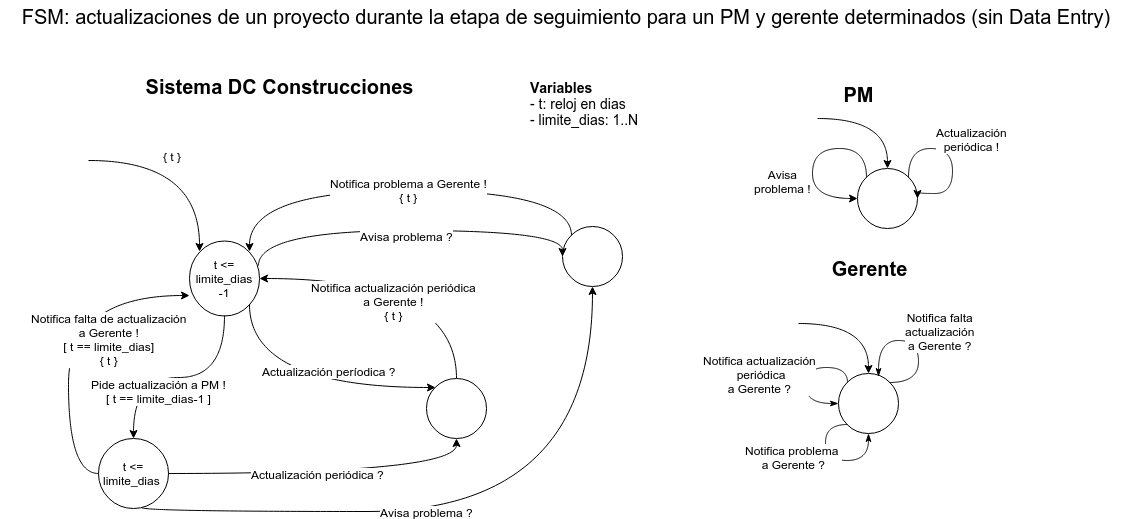
\includegraphics[scale=0.5, angle=90]{imagenes/FSM1.png}
\end{center}

\newpage
El segundo diagrama que mostraremos es el detalle del proceso mediante el cual el Cliente y el Gerente acuerdan el presupuesto a través del Sistema.

\begin{center}
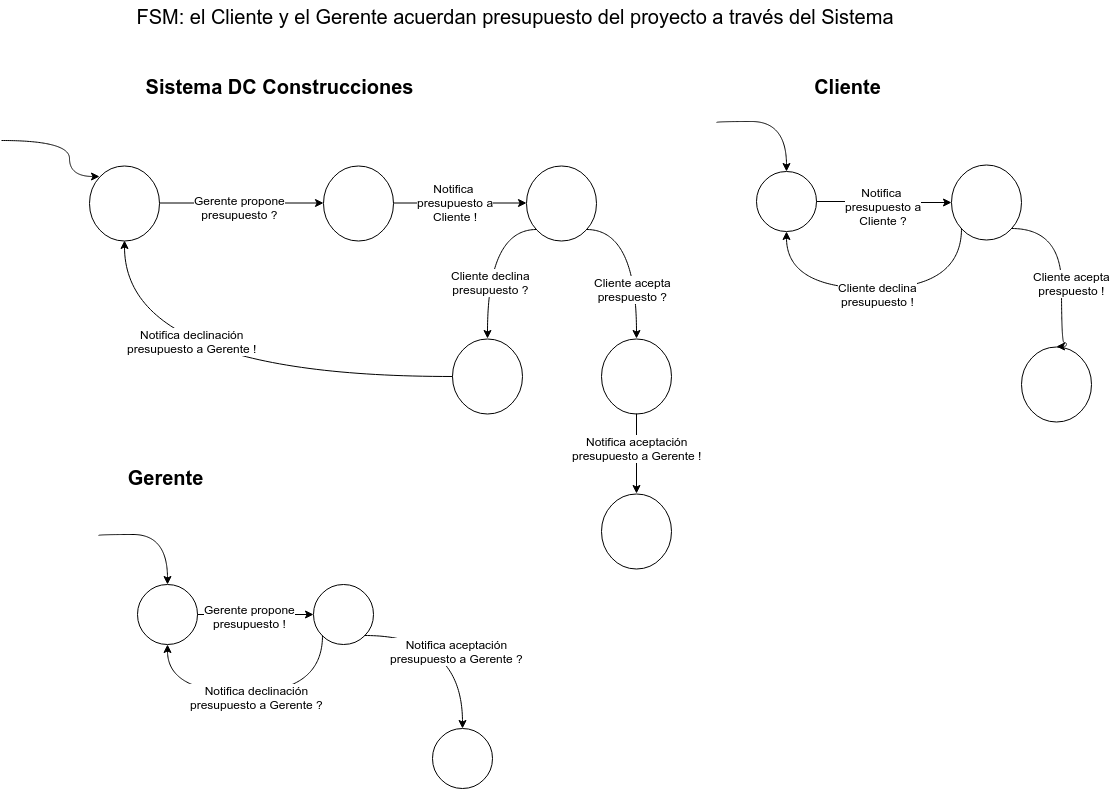
\includegraphics[scale=0.5, angle=90]{imagenes/FSM2.png}
\end{center}

\newpage
El tercer diagrama que mostraremos es el detalle del proceso mediante el cual el Cliente y el PM acuerdan el alcance del proyecto a través del Sistema.

\begin{center}
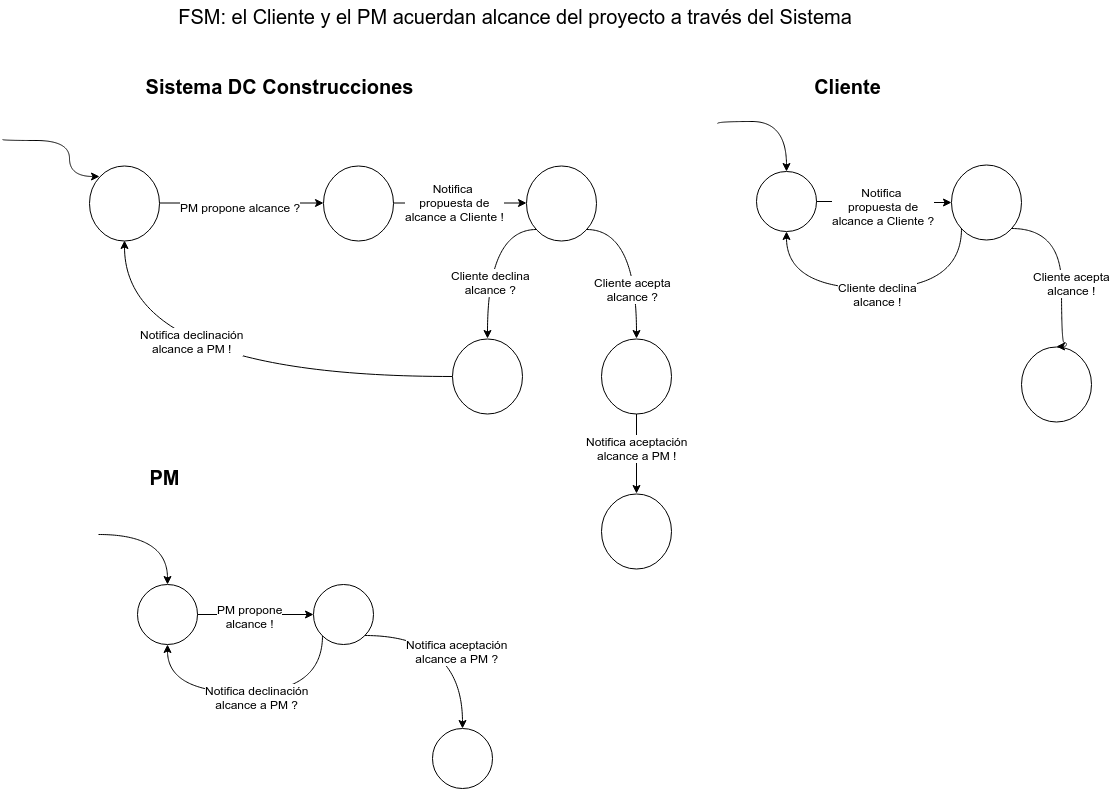
\includegraphics[scale=0.5, angle=90]{imagenes/FSM3.png}
\end{center}
